\documentclass[12pt]{kiarticle} % You can learn about my document class "kiarticle" and install it to your device by following the link: https://github.com/Kiarendil/toolkitex
\graphicspath{{pictures/}}
\DeclareGraphicsExtensions{.pdf,.png,.jpg,.eps}
%%%
\pagestyle{fancy}
\fancyhf{}
%\renewcommand{\headrulewidth}{ 0.1mm }
\renewcommand{\footrulewidth}{ .0em }
\fancyfoot[C]{\texttt{\textemdash~\thepage~\textemdash}}
\fancyhead[L]{Лабораторная работа № 3.4.2 \hfil}
\fancyhead[R]{\hfil Иванов Кирилл, 625 группа }

\newcommand
{\un}[1]
{\ensuremath{\text{#1}}}



\begin{document}

\begin{titlepage}
	\begin{center}
		\large 	Московский физико-технический университет \\
		Факультет общей и прикладной физики \\
		\vspace{0.2cm}
		
		\vspace{4.5cm}
		Лабораторная работа № 3.4.2 \\ \vspace{0.2cm}
		\large (Общая физика: электричество и магнетизм) \\ \vspace{0.2cm}
		\LARGE \textbf{Закон Кюри-Вейса}
	\end{center}
	\vspace{2.3cm} \large
	
	\begin{center}
		Работу выполнил: \\
		Иванов Кирилл,
		625 группа
		

		
		
	\end{center}
	
	\begin{center} \vspace{50mm}
		г. Долгопрудный \\
		 2017 год
	\end{center}
\end{titlepage}

%%%%%%%%%%
%%%%%%%%%%
%%%%%%%%%%%%%%%%%%%%%%%%%%%%%%%%%%%
\paragraph*{Цель работы:} изучение температурной зависимости магнитной восприимчивости ферромагнетика выше точки Кюри.

\paragraph*{Оборудование:} катушка самоиндукции с образцом из гадолиния, термостат, частометр, цифровой вольтметр, $ LC $-автогенератор, термопара медь-константин.


\section{Историческая справка}

Ферромагнетики обладают свойством намагничиваться даже в слабых магнитных полях. Впервые количественную теорию ферромагнетизма разработал французский физик Вейсс в 1907 году. В настоящей работе для изучения температурной зависимости магнитной восприимчивости ферромагнетика выше точки Кюри (то есть в парамагнитной области) используется закон Кюри-Вейса (который назван так по аналогии с законом Кюри для парамагнетиков).

Закон выражается следующей математической формулой:

 \begin{equation}\label{QW}
 \chi ={\frac  {C}{T-\Theta_p}} \sim \frac{1}{T - \Theta_p}, 
 \end{equation}
 
где $ \chi  $ — магнитная восприимчивость, $ С $ — постоянная Кюри, зависящая от вещества, $ T $ — абсолютная температура в кельвинах, $ \Theta_p  $ — парамагнитная температура Кюри, К.

\section{Теоретическое введение}

При повышении температуры $ Т $ возрастает дезориентирующее действие теплового движения частиц, и магнитная восприимчивость парамагнетиков
убывает, в простейшем случае (в постоянном магнитном
поле) - пo закону Кюри.

\begin{wrapfigure}{l}{0.4\linewidth} 
	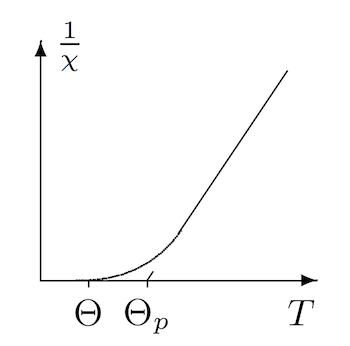
\includegraphics{342_gr}
	\caption{Теоретический график зависимости обратной магнитной восприимчивости от температуры}
\end{wrapfigure}

При $ Т \to 0 $ тепловое движение всё меньше препятствует магнитным моментам атомов ориентироваться в одном направлении при сколь
угодно слабом внешнем поле. В ферромагнетиках (под влиянием обменных сил) это происходит при понижении температуры не до абсолютного
нуля, а до температуры Кюри $ \Theta $, в котором добавка к температуре $ \Theta_p $ --- некая температура, называемая парамагнитной точкой Кюри. Она близка к $ \Theta $, но немного больше ее (см. рис.1). Оказывается, что у ферромагнетиков закон Кюри должен быть заменён законом Кюри-Вейсcа \eqref{QW}. Эта формула хорошо описывает поведение ферромагнитных  веществ после их перехода в парамагнитную фазу при заметном удалении температуры от 0 , но недостаточно точна при $ Т \approx \Theta$.

В нашей работе изучается температурная зависимость $ \chi(Т) $ гадолиния
при температурах выше точки Кюри. Выбор материала определяется
тем, что его точка Кюри лежит в интервале комнатных температур.

\section{Экспериментальная установка} 
\begin{figure}[h!]
	\centering
	\includegraphics[width=\linewidth]{pictures/342_stand}
	\caption{Схема эксперементальной установки}
	\label{fig:342stand}
\end{figure}

%\begin{wrapfigure}{l}{\linewidth} 
%	\includegraphics{342_stand}
%	\caption{Cхема экспериментальной установки}
%\end{wrapfigure}
Схема установки для проверки закона Кюри-Вейсса показана на рис. 2. Исследуемый ферромагнитный образец (гадолиний) расположен внутри пустотелой катушки самоиндукции, которая служит индуктивностью колебательного контура, входящего в состав $ LС $-автогенератора. 

Гадолиний является хорошим проводником электрического тока, а рабочая
частота генератора достаточно велика (50 кГц), поэтому для уменьшения
вихревых токов образец из готовлен из мелких кусочков размером 0,5 мм.
Катушка 1 с образцом помещена в стеклянный сосуд 2, залитый трансформаторным маслом. Масло предохраняет образец от окисления и способствует ухудшению электрического контакта между отдельными частичками образца. Кроме того, оно улучшает тепловой контакт между образцом и термостатируемой (рабочей) жидкостью 3 в термостате. Ртутный термометр 4 используется для приближенной оценки температуры.
При изменении температуры меняется магнитная восприимчивость образца
$ \chi $, а следовательно, самоиндукция катушки и период колебаний $ \tau $ автогенератора. Для измерения периода используется частотомер.

Закон Кюри- Вейсса справедлив, если выполнено соотношение

\begin{equation}\label{}
\dfrac{1}{\chi} \sim T - \Theta_p \sim \dfrac{1}{\tau^2 - \tau^2_0}
\end{equation}
где $ \tau_0 $ --- период колебаний без образца. 

Для нагрева используется термостат. Температура исследуемого образца всегда несколько отличается от температуры дистиллированной воды в сосуде. После того как вода достигла заданной температуры, идёт медленный процесс выравнивания температур образца и воды. Разность их температур контролируется с помощью медноконстантановой термопары 6 и цифрового вольтметра. Один из спаев термопары находится в тепловом контакте с образцом , а другой погружён в воду. Концы термопары подключены к цифровому вольтметру. Рекомендуется измерять период колебаний автогенератора в тот момент, когда указанная
разность температур становится $  \leq 0,5 \; ^\circ С $. Чувствительность термопары $ k= 24 $ град/мВ.

\section{Ход работы}

Запишем данные установки: $ k= 24 $ град/мВ, $ \tau_0 = 6,95636 $ мкс, $ \sigma_{\varDelta U} = 0,012 $ мВ, $ \sigma_{T_в} \hm{=}0,1 ^\circ C, \sigma_\tau = 0,01 $ мкс. Так как нам нужно, чтобы разница была не более половины градуса, то мы вычисляем максимальное напряжение, при котором допустимо измерение:

\begin{equation}\label{}
U_m = \dfrac{T_d}{k} = \dfrac{0,5}{24} \approx 0,021 \un{мВ} 
\end{equation}

Теперь снимем показания вольтметра и частометра при температуре термостата равной 14 $ ^\circ C $, и проведем такой опыт при 14 разных температурах, повышая после каждого измерения температуру термостата на два градуса. При этом температуру образца будем считать по следующей формуле:

\begin{equation}\label{}
T_o = T_в + \varDelta Uk
\end{equation}

Результаты занесем в таблицу \ref{res}.

\begin{table}[htbp]
	\centering
	\caption{Результаты измерений}

\begin{tabular}{|c|c|c|c|c|c|c|} 
	\hline 
	№ &  $ T_в $, $ ^\circ C $ &  $ \varDelta  U $, мВ & $ T_o $, $ ^\circ C$ & $ \tau, $ мкс & $ \tau^2 - \tau_0^2 $, $ мкс^2 $ & $ \dfrac{1}{\tau^2 - \tau_0^2} $, $ мкс^{-2} $  \\ 	\hline
	
%& \text{T$\_\unicode{0432}$} & \text{dU} & \text{T$\_$o} & \text{sigmaT$\_$o} & \text{$\backslash \backslash $tau} & \text{tDiff} &
%\text{sigmatDiff} & \text{tDiffRev} & \text{sigmatDiffRev} \\
 1. & 14.23 & 0.001 & 14.254 & 7.937 & 14.605 & 0.068 \\
2. & 16.12 & -0.017 & 15.712 & 7.872 & 13.577 & 0.074 \\
3. & 18.12 & -0.018 & 17.688 & 7.755 & 11.749 & 0.085 \\
4. & 20.1 & -0.018 & 19.668 & 7.568 & 8.884 & 0.113 \\
5. & 22.1 & -0.017 & 21.692 & 7.358 & 5.749 & 0.174 \\
6. & 24.11 & -0.018 & 23.678 & 7.193 & 3.348 & 0.299 \\
7. & 26.08 & -0.018 & 25.648 & 7.121 & 2.318 & 0.431 \\
8. & 28.1 & -0.012 & 27.812 & 7.079 & 1.721 & 0.581 \\
9. & 30.09 & -0.017 & 29.682 & 7.055 & 1.382 & 0.724 \\
10. & 32.08 & -0.018 & 31.648 & 7.036 & 1.114 & 0.897 \\
11. & 34.08 & -0.017 & 33.672 & 7.022 & 0.918 & 1.09 \\
12. & 36.09 & -0.019 & 35.634 & 7.013 & 0.791 & 1.264 \\
13. & 38.08 & -0.018 & 37.648 & 7.005 & 0.679 & 1.473 \\
14. & 40.08 & -0.019 & 39.624 & 6.999 & 0.595 & 1.681 \\
	\hline

\end{tabular}% 
\label{res}% 
\end{table}% 

\begin{wraptable}{l}{0.5\linewidth}
	\caption{Погрешности}
	\begin{tabular}{|c|c|c|c|}
		\hline
		\text{№} & $ \sigma_{T_o}  $ & $  \sigma_{\tau^2 - \tau_0^2} $ $,  мкс^{2}  $ &  $ \sigma_{\frac{1}{\tau^2 - \tau_0^2}} $, $ мкс^{-2}  $ \\
		\hline
		1. & 0.10 & 0.159 & 0.001 \\
		2. & 0.10 & 0.157 & 0.001 \\
		3. & 0.10 & 0.155 & 0.001 \\
		4. & 0.10 & 0.151 & 0.002 \\
		5. & 0.10 & 0.147 & 0.004 \\
		6. & 0.10 & 0.144 & 0.013 \\
		7. & 0.10 & 0.142 & 0.027 \\
		8. & 0.10 & 0.142 & 0.048 \\
		9. & 0.10 & 0.141 & 0.074 \\
		10. & 0.10 & 0.141 & 0.113 \\
		11. & 0.10 & 0.14 & 0.13 \\
		12. & 0.10 & 0.14 & 0.152 \\
		13. & 0.10 & 0.14 & 0.185 \\
		14. & 0.10 & 0.14 & 0.211 \\
		\hline
	\end{tabular}
\end{wraptable}
Посчитаем погрешности: 

$$
\sigma_{T_o} = \sqrt{\sigma_{T_в}^2 + \sigma_{dUk}^2}
$$
\begin{equation}\label{}
\sigma_{\tau^2 - \tau_0^2} = \dfrac{d(\tau^2 - \tau_0^2)}{d\tau}\sigma_\tau = 2\tau\sigma_\tau
\end{equation}
\begin{equation}\label{}
\sigma_{\frac{1}{\tau^2 - \tau_0^2}} = \dfrac{d\s{\dfrac{1}{\tau^2 - \tau_0^2}}}{d\tau}\sigma_\tau = \dfrac{2\tau}{{(\tau^2 - \tau_0^2)^2}}\sigma_\tau
\end{equation}

По результатам вычисления погрешностей составим таблицу 2.

На основе таблиц 1 и 2 построим графики зависимости величин $ \tau^2 - \tau_0^2 $ и $ \dfrac{1}{\tau^2 - \tau_0^2} $ от температуры образца.
\par
На графике рис. 3 проведем прямую через последние 7 точек и аппроксимируем ее к оси абсцисс. Результаты занесем в таблицу 3.

На графике рис.4 видно, что наблюдается излом в райне третей точки графика. 
\vspace{1mm}
\begin{figure}[h!]
	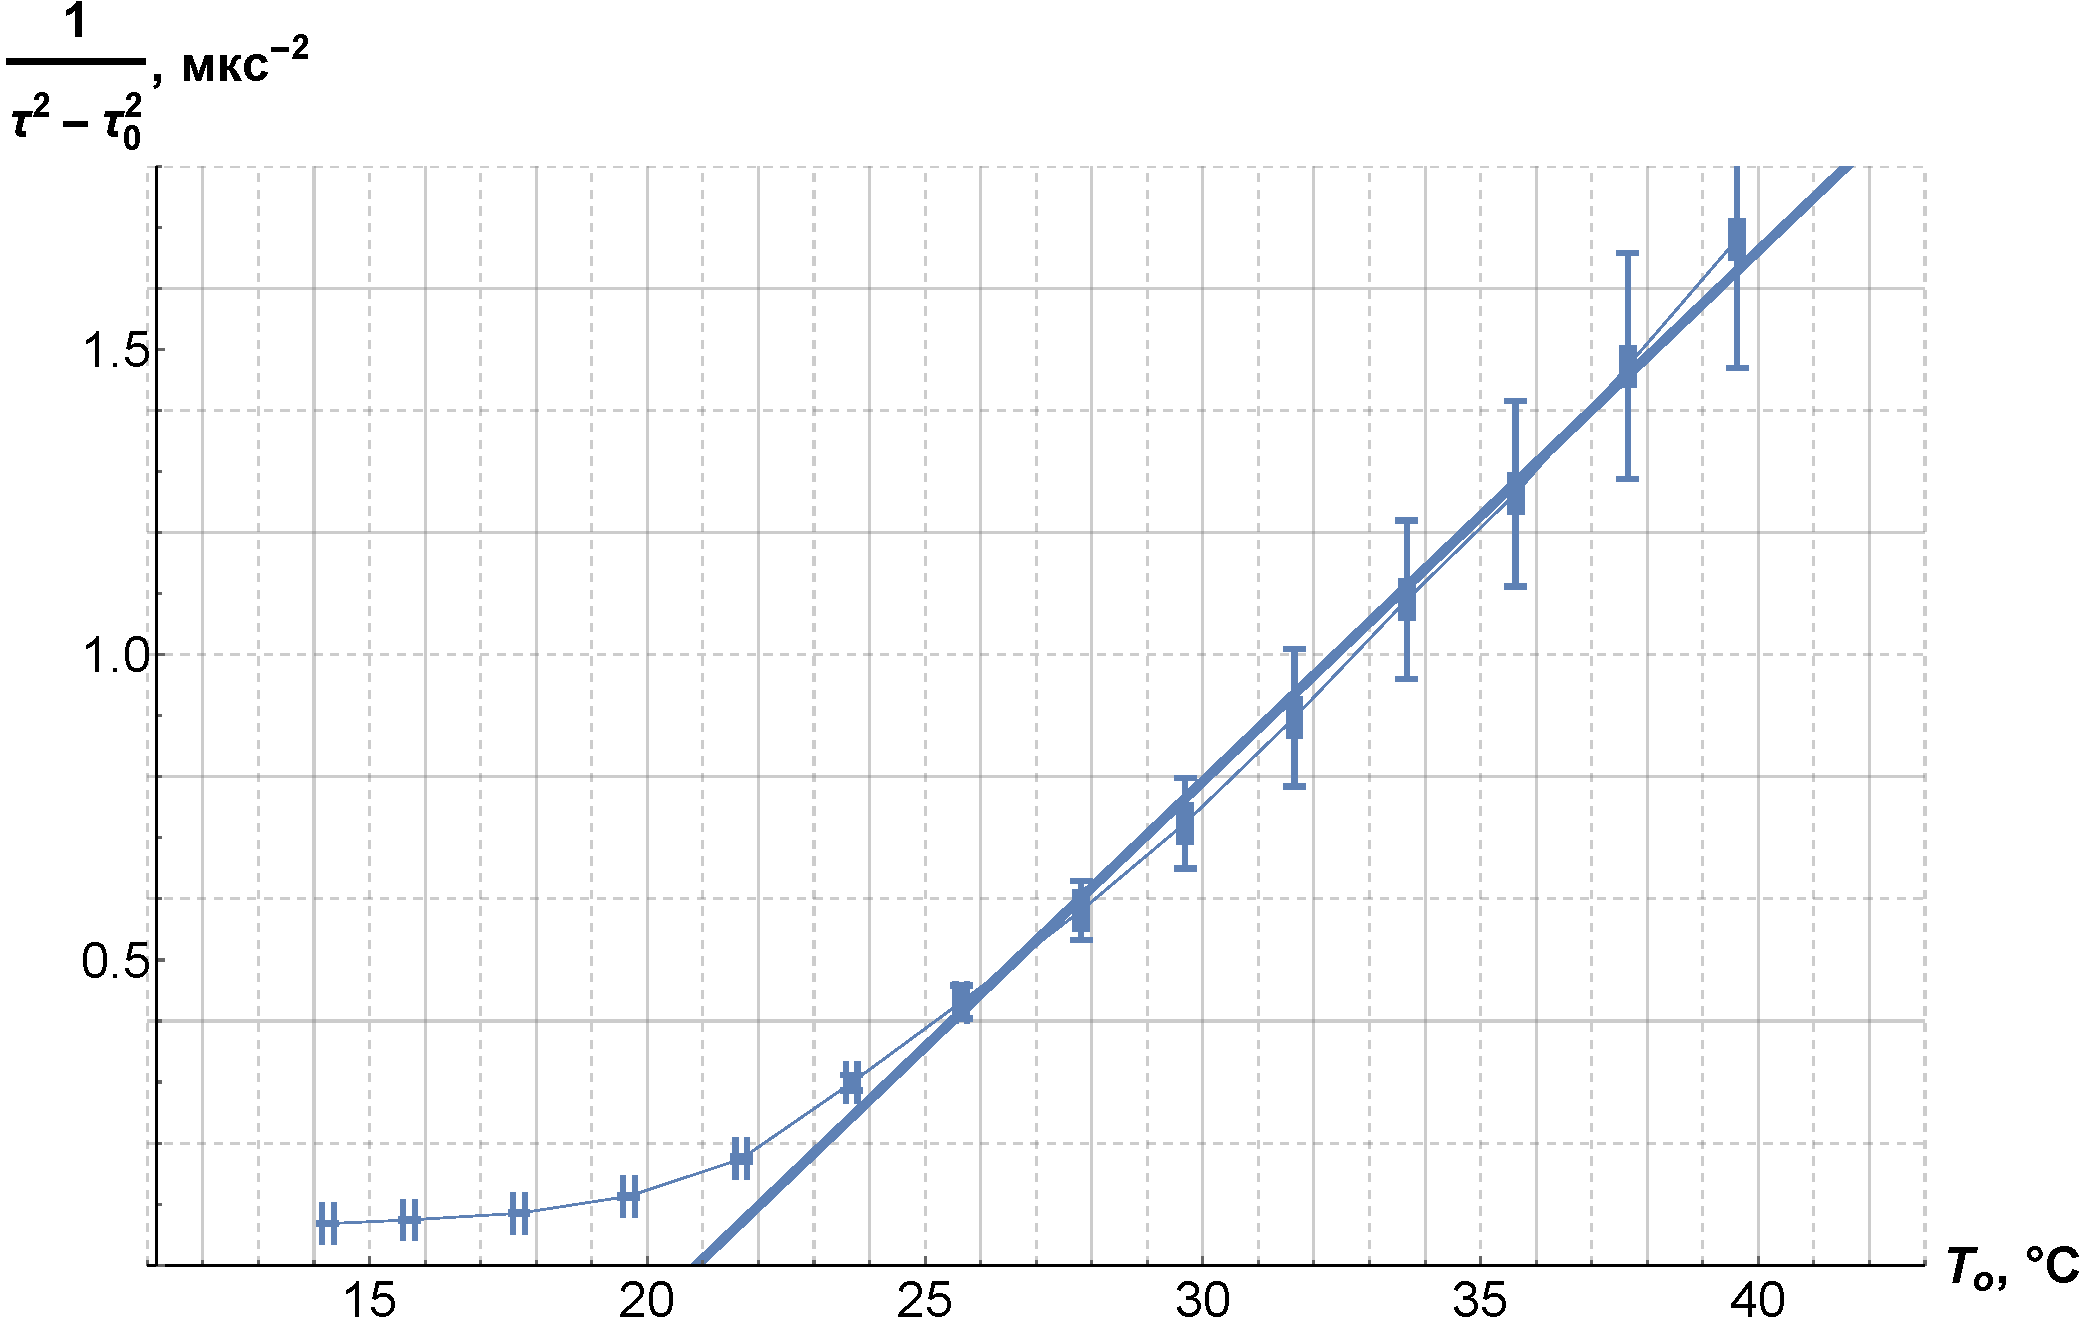
\includegraphics[scale=0.47]{rev.pdf}
	\caption{Зависимость $ \dfrac{1}{ \tau^2 - \tau_0^2} $ от температуры образца}
\end{figure}
\begin{table}%{l}{0.5\linewidth}
	\centering
	\caption{Расчет апроксимированной прямой $ y = ax +b $}
	\begin{tabular}{c|cc}
		\text{} & \text{Estimate} & \text{Standard Error} \\
		\hline
		b & -1.816 & 0.082  \\
		a & 0.087 & 0.002  \\
	\end{tabular}
\end{table}


Таким образом, это и есть искомая точка Кюри $ \Theta $, которая наблюдается в ожидаемом для нее месте (согласно табличным данным, $ \Theta = 16 \; ^\circ C $). На графике рис.3 видно, что график превращается в почти параллельную оси абсцисс прямую, близкую к нулю, также в районе $ 16 \; ^\circ C $.

По результатам таблицы 3 получаем прямую 

\begin{equation}\label{}
 \dfrac{1}{ \tau^2 - \tau_0^2} = 0,087\x T_o - 1,816
\end{equation}

При 0 по оси ординат парамагнитная температура Кюри $ \Theta_p = \dfrac{1,1816}{0,087} \approx 20,83 \; ^\circ C$. Погрешность полученной величины

\begin{equation}\label{}
\sigma_{\Theta_p} = \Theta_p \sqrt{\s{\dfrac{\sigma_a}{a}}^2 + \s{\dfrac{\sigma_b}{b}}}^2 = 1,05 ^\circ C
\end{equation}

\section{Вывод}

По результатам проделанной работы мы высчитали парамагнитную точку Кюри для гадолиния:

\begin{center}
	{\fbox{ $ \Theta_p = (20,83 \pm 1,05) \; ^\circ C$}} \\
\end{center} 

Как и предполагалось в теоретическом введении, эта температура выше обычной точки Кюри, которая примерно равна 16--17 $ ^\circ C $. 

Полученный результат достаточно хорошо согласуется с табличными данными, где точка Кюри гадолиния $ \Theta_т = 16 \; ^\circ C $.

\end{document}